\chapter{Introduction}
\label{cha:introduction}

This chapter presents the overview and general objectives of the thesis.
The first section describes the motivations for the project. Different
approaches to the problem are presented in the next section. Finally,
in the last two sections the VPH-Share Cloud Platform context is introduced
and high-level objectives of this thesis are presented.
 
\section{Background and overview}
In the modern world of the 21st century the data and its vast volume
is ubiquitous. The total amount of global data stored to date is estimated
as 2.7 zettabytes ($2.7 \times 10^{21}bytes$). As long as computers
become more common and excellent and enter new domains, the exponential
growth of data volume will continue. The main sources of data are
of various kind:

\begin{itemize}
\item \textbf{personal data} -- generated by and associated with people such as
images, videos, emails, documents etc, stored on privately held devices as
laptops, smartphones or digital cameras as well as by website owners in
big data centers,
\item \textbf{business data} -- generated by companies and corporations
that enables them to run and maintain their daily business,
\item \textbf{experimental data} -- generated by all kind of sensor and
experimental devices from weather stations, to particle accelerators, to
space satellites and stored on academic resources and scientific data centers.
\end{itemize}

It is an engineering challenge to fullfill storage requirements for current
data growth. Nowadays, we observe a rapid shift from privately owned and maintained
computer systems toward virtualized computer infrastructures provided as a service,
namely cloud computing. At least several commercial cloud infrastructure offerings 
provide access to virtualized computer systems at different level -- Infrastructure
as a Service (IaaS), Platform as a Service (PaaS) and Software as a Service (SaaS).
Low costs, high availability and scalability, decent performance degradation and 
seamless integration are often mentioned as major benefits by cloud adopters.\\

Digitalization brought new opportunities and benefits to the business world.
However, it caused a lot of companies to depend on their data. At this point,
company's data is often the biggest asset and a complete data loss results in 
business failure. Temporal data unavailability can also pose a problem in domains
such as medical care and flight services. As a result, data loss prevention appears
everywhere where valuable data exists, from backups, to data replication. Ideally,
from the user point of view, data storage solution should:

\begin{enumerate}
\item provide highly available access to the data,
\item provide fault-tolerant storage of the data,
\item be free of data corruption and integrity problems.
\end{enumerate}

However, it often appears that the above-mentioned criteria cannot be met,
especially when relying on single service provider. Cloud service providers protect
their customers data with data replication to geographically distributed zones,
strong securitiy policies and infrastructure monitoring. Even though, recently
a~number of cloud failures occured, questioning the reliability of
cloud solutions. Malicious and accidental data corruption threats also require
attention. There is a standard concept of data integrity verification which consists
of two major steps -- initial setup and verification. The first step concerns
initial data deployment and integrity metadata -- mostly hash checksums -- of the
content computed. In the verification step the integrity checksums are once more
computed and compared with the reference ones.\\

Managing the risk and reliability of cloud storage environment is the subject of this
thesis. To address the problem the idea is to build another abstraction layer on top
of cloud service and be able to use multiple cloud providers interchangeably, so called
federated cloud storage. With federated approach we can easily detect cloud provider
failure and switch to another. However, data corruption still poses a problem. Apart
from data replication between cloud providers it is necessary to periodically monitor
the integrity of stored data and proactively restore corrupted entities from existing
replicas or notify the user about data corruption.

Summing up the above considerations, the objective of this thesis is to create a tool
in the form of a service that will:

\begin{enumerate}
\item continuously and periodically monitor the integrity of the data stored in the
federation of cloud storage resources,
\item proactively restore discovered data corruption from the replicas in other cloud
providers,
\item notify the data owner(user) about discovered data corruption in advance of data retrieval. 
\end{enumerate}

\section{Cloud storage data reliability challenges}
Data reliability is a must-have requirement is today's computer systems. In many areas
of science, business and culture computers already play a crucial role. In this thesis
by data reliability we mean both:

\begin{enumerate}
\item \textbf{availability} -- that the data is available to the requesting entity,
\item \textbf{integrity} -- that the data remains untouched by malicious or undesired
modifications.
\end{enumerate}

These two ingredients are required, as corrupted or unavailable data makes it useless
or even harmful. We can distinguish two aspects of ensuring data reliability --
detection and recovery. Corruption or unavailability detection helps us to spot data
problems, while recovery enables us to retrieve from them. Computer industry developed
number of methods -- from hash-based checksums in software distribution, to error correcting
codes in hardware, to automatic replication and backup. These methods provide a solid
background, however, as computing paradigms evolve, they can become obsolete.\\

While emerging cloud storage trend determines a significant step forward and brings a lot
of advantages as data replication, no administration costs, pay-as-you-use, SLA contracts 
-- it can appear challenging for ensuring data reliability. Recent cloud storage failure
or security break reports shown that we cannot entrust our data to cloud providers entirely
-- data reliability still requires monitoring. However, classic checksum-based integrity
verfication of vast volumes of data stored on remote resources, where network transfer
rates and latency comes into play, is unacceptable. Additionally, cloud storage providers
charge fees not only for storage space used, but also for storage transfer. As a result,
researchers and engineers search for methods that would enable corruption detection
based on a fraction of file's content with high probability. A part of this thesis main
objective is to select and implement a network-efficient method of ensuring data availability
and integrity.

 

\section{VPH-Share Cloud Platform context}
This thesis originates as a part of the VPH-Share project founded by European Commission
which brings together twenty international partners from academia, industry and healthcare,
led by University of Sheffield. Its main goal is to build a collaborative computing
environment and infrastructure where researchers from the domain oh physiopathology of
the human body will work together on developing new medical simulation software. The inspiring
vision is to create a versatile environment for sharing of information -- tools, models and data
-- to work efficiently towards building a complete model of the human body.\\

The project has layered architecture divided into work packages distributed among consortium
members (see figure \ref{fig:dri-high-level}). The design is based on cloud computing middleware
-- a hybrid of commercial and private resources on top of hardware layer. Data and Compute
Cloud Platform is one of the main building blocks of the VPH-Share project. Its goal is to
develop and integrate a consistent service-based cloud infrastructure that will enable VPH
community to deploy basic components of VPH-Share application workflows (known as Atomic Services)
on the available computing resources and then enact workflows using these services. Access to the
services layer will be provided to system users through user interface(UI).

\begin{figure}[h!]
	\centering
	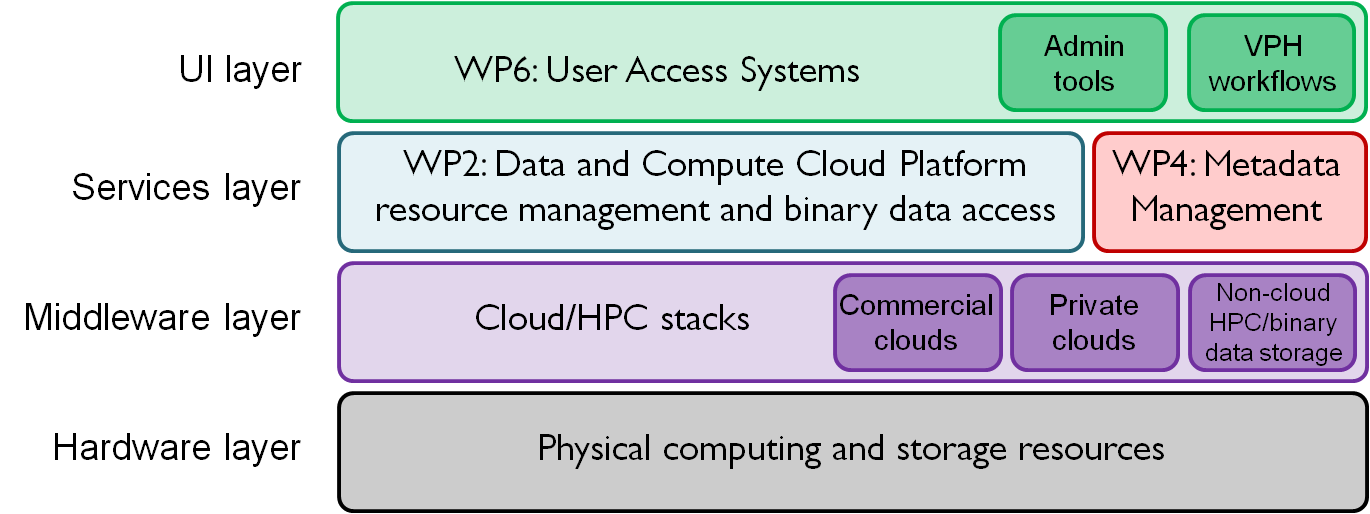
\includegraphics[width=0.8\textwidth]{images/vph-high-level.png}
	\caption{VPH-Share overview: Data and Compute Cloud Platform in layered VPH-Share architecture}
	\label{fig:dri-high-level}
\end{figure} 


VPH-Share specifies three groups of users:
application providers, domain scientists and system administrators. Application providers
are responsible for developing and installing scientific applications and software packages.
Domain scientists are actual researchers of VPH community who will use and benefit from 
the platform. Finally, system administrators is a group of priviledged users who will
manage platform's hardware resources and will administer and maintain it.\\

According to the platform's design, data will be stored on federated cloud storage resources --
both commercial and private -- and available via common access layer. It is foreseen that stored
data volumes will be significant, but predominantly of static nature -- upon upload its content will
remain untouched. Additional measures should ensure data availability and integrity.As a result, two
of the key project's requirements regarding data storage and integrity are:

\begin{itemize}
\item \textbf{access to large binary data in the cloud} -- specified groups of users will
be able to query for and store binary data uploaded or generated by workflows within the platform, 
\item \textbf{data reliability and integrity} -- platform users will be able to tag datasets
for automatic availability and integrity monitoring, set validation and replication policies,
as well as receive notifications about data integrity violations.
\end{itemize}




\section{Objectives of this work}
